%%%%%%%%%%%%%%%%%%%%%%%%%%%%%%%%%%%%%%%%%%%%%%%%%%%%%%%%%%%%%%%%%%%%%%%%%%%%%%%%
% TUM-Vorlage: Präsentation
%%%%%%%%%%%%%%%%%%%%%%%%%%%%%%%%%%%%%%%%%%%%%%%%%%%%%%%%%%%%%%%%%%%%%%%%%%%%%%%%
%
% Rechteinhaber:
%     Technische Universität München
%     https://www.tum.de
% 
% Gestaltung:
%     ediundsepp Gestaltungsgesellschaft, München
%     http://www.ediundsepp.de
% 
% Technische Umsetzung:
%     eWorks GmbH, Frankfurt am Main
%     http://www.eworks.de
%
%%%%%%%%%%%%%%%%%%%%%%%%%%%%%%%%%%%%%%%%%%%%%%%%%%%%%%%%%%%%%%%%%%%%%%%%%%%%%%%%


%%%%%%%%%%%%%%%%%%%%%%%%%%%%%%%%%%%%%%%%%%%%%%%%%%%%%%%%%%%%%%%%%%%%%%%%%%%%%%%%
% Zur Wahl des Seitenverhältnisses bitte einen der beiden folgenden Befehle
% auskommentieren und den ausführen lassen:
\input{./Ressourcen/Praesentation/Praeambel4zu3.tex} % Seitenverhältnis 4:3
% \input{./Ressourcen/Praesentation/Praeambel16zu9.tex} % Seitenverhältnis 16:9
%%%%%%%%%%%%%%%%%%%%%%%%%%%%%%%%%%%%%%%%%%%%%%%%%%%%%%%%%%%%%%%%%%%%%%%%%%%%%%%%


%%%%%%%%%%%%%%%%%%%%%%%%%%%%%%%%%%%%%%%%%%%%%%%%%%%%%%%%%%%%%%%%%%%%%%%%%%%%%%%%
\input{./_Einstellungen.tex}                    % !!! DATEI ANPASSEN !!!
%%%%%%%%%%%%%%%%%%%%%%%%%%%%%%%%%%%%%%%%%%%%%%%%%%%%%%%%%%%%%%%%%%%%%%%%%%%%%%%%
\usepackage{tikz}
\usepackage{amsmath}
\usepackage{relsize}
\usepackage{amssymb}
\usepackage{mathtools}
\usepackage{algorithm}
\usepackage{algpseudocode}
\usepackage{subfigure}
\usetikzlibrary{shapes.geometric, arrows, backgrounds, calc, positioning, decorations.pathreplacing, calligraphy}

\renewcommand{\PersonTitel}{B.Sc.}
\renewcommand{\PersonVorname}{Jonas}
\renewcommand{\PersonNachname}{Schulz}
%\renewcommand{\FakultaetName}{Department of Informatics}
\renewcommand{\LehrstuhlName}{@ Chair of Algorithms and Complexity}
%\renewcommand{\UniversitaetName}{Technical University of Munich}
\newcommand{\Datum}{19.12.2022}

\renewcommand{\PraesentationFusszeileZusatz}{| Master's Colloquium | An Experimental Evaluation of Heuristics for Approx. Maxflow Alg.}

\title{Master's Colloquium}
\author{\PersonTitel{} \PersonVorname{} \PersonNachname}
\institute[]{\UniversitaetName \\ \FakultaetName}
%\institute[]{\UniversitaetName \\ \FakultaetName \\ \LehrstuhlName}
\date[\Datum]{München, 19.12.2022}
\subject{An Experimental Evaluation of Heuristics for Approximate Maxflow Algorithms}


%%%%%%%%%%%%%%%%%%%%%%%%%%%%%%%%%%%%%%%%%%%%%%%%%%%%%%%%%%%%%%%%%%%%%%%%%%%%%%%%
\input{./Ressourcen/Praesentation/Anfang.tex} % !!! NICHT ENTFERNEN !!!
%%%%%%%%%%%%%%%%%%%%%%%%%%%%%%%%%%%%%%%%%%%%%%%%%%%%%%%%%%%%%%%%%%%%%%%%%%%%%%%%


%%%%%%%%%%%%%%%%%%%%%%%%%%%%%%%%%%%%%%%%%%%%%%%%%%%%%%%%%%%%%%%%%%%%%%%%%%%%%%%%
% FOLIENSTIL: Standard
\PraesentationMasterStandard
\PraesentationTitelseite % Fügt die Startseite ein




%%%%%%%%%%%%%%%%%%%%%%%%%%%%%%%%%%%%%%%%%%%%%%%%%%%%%%%%%%%%%%%%%%%%%%%%%%%%%%%%
% FOLIENSTIL: Weisse Schrift auf blauem Grund
%\PraesentationMasterWeissBlau

%%%%%%%%%%%%%%%%%%%%%%%%%%%%%%%%%%%%%%%%%%%%%%%%%%%%%
%% Startseiten                                     %%

% Setzt die Startseite auf eine mit Flaggen als Hintergrund:
%\PraesentationStartseiteFlaggen

% Setzt die Startseite auf eine mit mit einer Zeichnung des TUM-Uhrenturms:
%\PraesentationStartseiteUhrenturm

% Setzt die Startseite auf eine ohne Hintergrund:
%\PraesentationStartseiteLeer

%\PraesentationTitelseite % Fügt die Startseite ein
%%%%%%%%%%%%%%%%%%%%%%%%%%%%%%%%%%%%%%%%%%%%%%%%%%%%%


\begin{frame}
    \PraesentationUeberschriftZweizeilig{Master's Colloquium}{An Experimental Evaluation of Heuristics for Approximate Maxflow Algorithms}
\end{frame}

%%%%%%%%%%%%%%%%%%%%%%%%%%%%%%%%%%%%%%%%%%%%%%%%%%%%%%%%%%%%%%%%%%%%%%%%%%%%%%%%
% FOLIENSTIL: Weisse Schrift auf schwarzem Grund
%\PraesentationMasterWeissSchwarz

%\begin{frame}
%    \frametitle{Introduction}
%    
%\begin{PraesentationAufzaehlung}
%\item<+(1)-> Hi
%\item<.(1)-> Hi 2
%\item<+(1)-> Hi 3
%\end{PraesentationAufzaehlung}
%
%\end{frame}
%\clearpage






\begin{frame}
\frametitle<.->{Maxflows: Runtimes}
\begin{itemize}
\item<+-> Directed Graph: $\color{blue}\mathcal{O}(m\cdot \min(m^{1/2},n^{1/3}))$ \textcolor{gray}{(Goldberg, Rao)}
\item<+-> Sparsification: $\color{blue}T(m,n)\rightarrow \mathcal{O}(m)+(m/n)\cdot T(\mathcal{O}(n),n))$ \textcolor{gray}{(Benczùr, Karger)}
\item<+-> Goldberg/Rao on sparsified graph (approximative): $\color{blue}\mathcal{O}(mn^{1/2})$
\item<+-> Christiano \textit{et al.} + Laplacian Solver (Spielman, Teng) (approximative): $\color{blue}\mathcal{O}(mn^{1/3})$
\item<+-> Sherman: Single-commodity flows (undirected graph, approximative): $(1+\varepsilon)$-optimal in $\color{blue}\mathcal{O}(m^{1+o(1)}\varepsilon^{-2})$
\end{itemize}
\end{frame}

\begin{frame}
\frametitle<.->{Maxflows}

\begin{center}
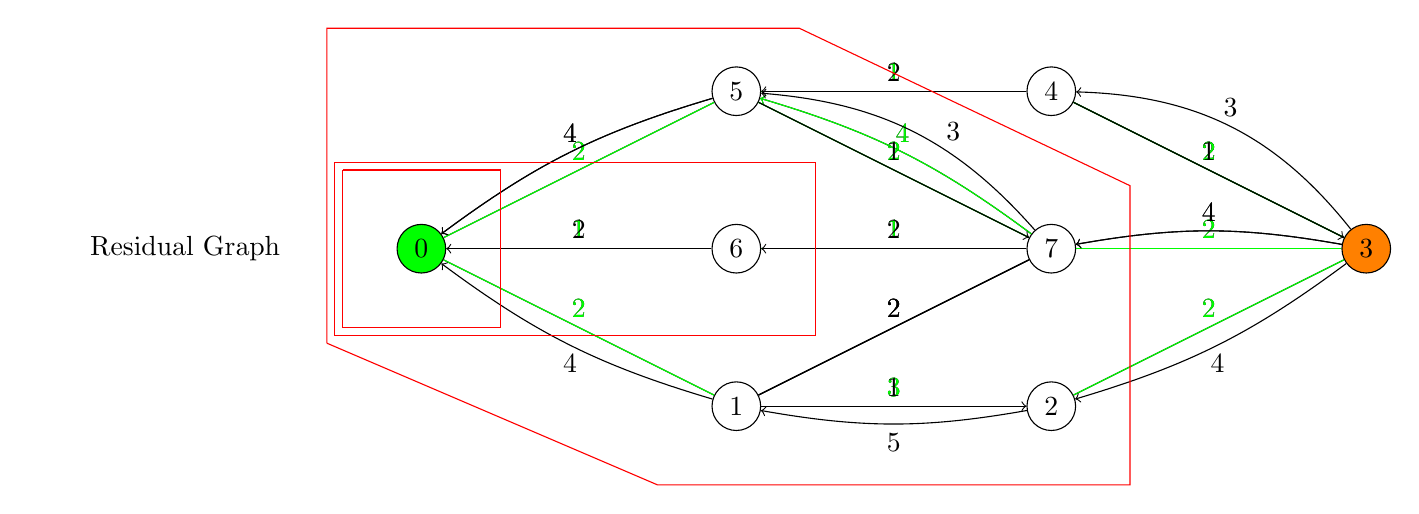
\begin{tikzpicture}
\node<.(1)-> at (-3,0) [minimum width=4cm] {Residual Graph};

\node<.(1)-> (0) at (0,0) [draw, circle, fill=green] {0};
\node<.(1)-> (1) at (4,-2) [draw, circle] {1};
\node<.(1)-> (2) at (8,-2) [draw, circle] {2};
\node<.(1)-> (3) at (12,0) [draw, circle, fill=orange] {3};
\node<.(1)-> (4) at (8,2) [draw, circle] {4};
\node<.(1)-> (5) at (4,2) [draw, circle] {5};
\node<.(1)-> (6) at (4,0) [draw, circle] {6};
\node<.(1)-> (7) at (8,0) [draw, circle] {7};
% step 1
\path<.(1)-.(3)>
    (0) edge node[above]{1} (6)
    (0) edge node[above]{2} (5)
    (6) edge node[above]{1} (7)
    (5) edge node[above]{1} (4)
    (4) edge node[above]{2} (3)
    (7) edge node[above]{2} (3)
    (1) edge node[above]{2} (7)
    (5) edge node[above]{2} (7);
\path<.(1)>
    (0) edge node[above]{2} (1)
    (1) edge node[above]{3} (2)
    (2) edge node[above]{2} (3);
\path<.(2)>
    (0) edge[green] node[above,color=green]{2} (1)
    (1) edge[green] node[above,color=green]{3} (2)
    (2) edge[green] node[above,color=green]{2} (3);
\path<.(3)->[->]
    (1) edge[bend left=10] node[below]{4} (0)
    (1) edge node[above]{1} (2)
    (2) edge[bend left=10] node[below]{5} (1)
    (3) edge[bend left=10] node[below]{4} (2);
% step 2
\path<.(4)-.(5)>
    (0) edge node[above]{1} (6)
    (6) edge node[above]{1} (7)
    (5) edge node[above]{1} (4)
    (4) edge node[above]{2} (3)
    (1) edge node[above]{2} (7);
\path<.(4)>
    (0) edge[green] node[above,color=green]{2} (5)
    (5) edge[green] node[above,color=green]{2} (7)
    (7) edge[green] node[above,color=green]{2} (3);
\path<.(5)>[->]
    (5) edge[bend right=10] node[above]{4} (0)
    (7) edge[bend right=10] node[above]{4} (5)
    (3) edge[bend right=10] node[above]{4} (7);
% step 3
\path<.(6)->
    (1) edge node[above]{2} (7)
    (5) edge[bend right=10,->] node[above]{4} (0)
    (3) edge[bend right=10,->] node[above]{4} (7);
\path<.(6)>
    (0) edge[green] node[above,color=green]{1} (6)
    (6) edge[green] node[above,color=green]{1} (7)
    (5) edge[green] node[above,color=green]{1} (4)
    (4) edge[green] node[above,color=green]{2} (3)
    (7) edge[green, bend right=10,->] node[above,color=green]{4} (5);
\path<.(7)->[->]
    (6) edge node[above]{2} (0)
    (7) edge node[above]{2} (6)
    (4) edge node[above]{2} (5)
    (4) edge node[above]{1} (3)
    (3) edge[bend right=25] node[above]{3} (4)
    (5) edge node[above]{1} (7)
    (7) edge[bend right=22] node[right=.3cm]{3} (5);
\draw<.(9)->[red] (-1,1) -- (-1,-1) -- (1,-1) -- (1,1) -- (-1,1);
\draw<.(10)->[red] (-1.1,1.1) -- (-1.1,-1.1) -- (5,-1.1) -- (5,1.1) -- (-1.1,1.1);
\draw<.(11)->[red] (-1.2,-1.2) -- (-1.2,2.8) -- (4.8,2.8) -- (9,0.8) -- (9,-3) -- (3,-3) -- (-1.2,-1.2);
\end{tikzpicture}
\end{center}

\begin{center}
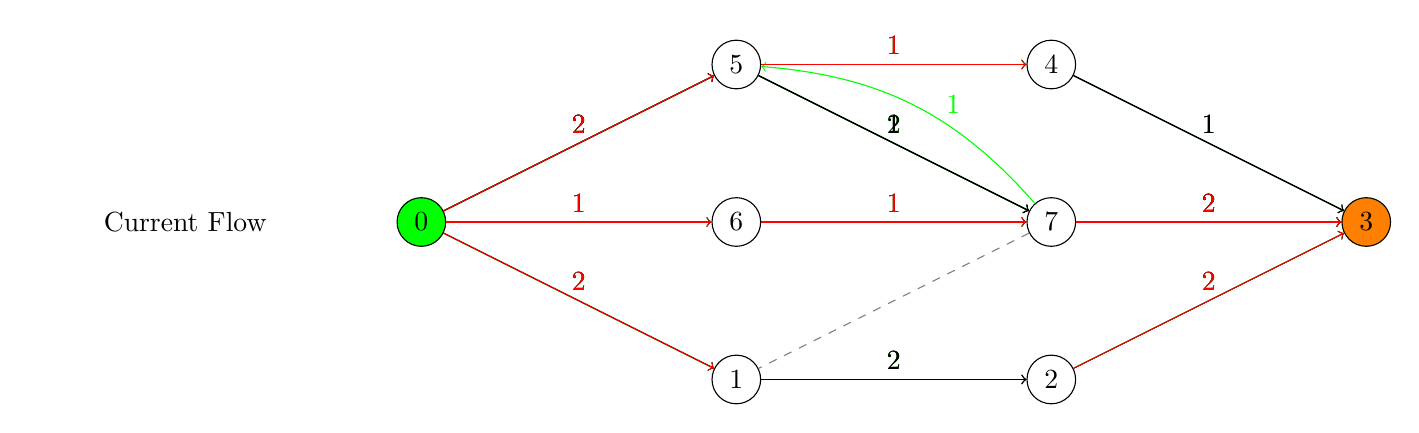
\begin{tikzpicture}
\node<.(1)-> at (-3,0) [minimum width=4cm] {Current Flow};

\node<.(1)-> (0) at (0,0) [draw, circle, fill=green] {0};
\node<.(1)-> (1) at (4,-2) [draw, circle] {1};
\node<.(1)-> (2) at (8,-2) [draw, circle] {2};
\node<.(1)-> (3) at (12,0) [draw, circle, fill=orange] {3};
\node<.(1)-> (4) at (8,2) [draw, circle] {4};
\node<.(1)-> (5) at (4,2) [draw, circle] {5};
\node<.(1)-> (6) at (4,0) [draw, circle] {6};
\node<.(1)-> (7) at (8,0) [draw, circle] {7};
% step 1
\path<.(2)>[->]
    (0) edge[green] node[above,color=green]{2} (1)
    (1) edge[green] node[above,color=green]{2} (2)
    (2) edge[green] node[above,color=green]{2} (3);
\path<.(3)-.(7)>[->]
    (0) edge node[above]{2} (1)
    (1) edge node[above]{2} (2)
    (2) edge node[above]{2} (3);
% step 2
\path<.(4)>[->]
    (0) edge[green] node[above,color=green]{2} (5)
    (5) edge[green] node[above,color=green]{2} (7)
    (7) edge[green] node[above,color=green]{2} (3);
\path<.(5)-.(6)>[->]
    (0) edge node[above]{2} (5)
    (5) edge node[above]{2} (7)
    (7) edge node[above]{2} (3);
% step 3
\path<.(6)>[->]
    (0) edge[green] node[above,color=green]{1} (6)
    (6) edge[green] node[above,color=green]{1} (7)
    (5) edge[green] node[above,color=green]{1} (4)
    (4) edge[green] node[above,color=green]{1} (3)
    (7) edge[green, bend right=22] node[right=.3cm,color=green]{1} (5);
\path<.(7)>[->]
    (0) edge node[above]{2} (5)
    (5) edge node[above]{1} (7)
    (7) edge node[above]{2} (3)
    (0) edge node[above]{1} (6)
    (6) edge node[above]{1} (7)
    (5) edge node[above]{1} (4)
    (4) edge node[above]{1} (3);
% marking all max congested edges
\path<.(8)->[->]
    (0) edge[red] node[above,color=red]{2} (1)
    (1) edge node[above]{2} (2)
    (2) edge[red] node[above,color=red]{2} (3)
    (0) edge[red] node[above,color=red]{2} (5)
    (5) edge node[above]{1} (7)
    (7) edge[red] node[above,color=red]{2} (3)
    (0) edge[red] node[above,color=red]{1} (6)
    (6) edge[red] node[above,color=red]{1} (7)
    (5) edge[red] node[above,color=red]{1} (4)
    (4) edge node[above]{1} (3)
    (7) edge[-,dashed,gray] (1);
\end{tikzpicture}
\end{center}
\end{frame}

\begin{frame}
\frametitle<.->{Minimum Congestion Flow}

\begin{itemize}
\item<+-> Maximum Flow Problem: 
\begin{itemize}
\item<+-> $s$-$t$-flow of maximal value
\item<+-> restricted to $s$-$t$-flows
\end{itemize}
\item<+-> Minimum Congestion Flow Problem:
\begin{itemize}
\item<+-> flow with minimal value of the \textit{\color{blue}maximum congestion}
\item<+-> \textit{\color{blue}maximum congestion}: $\max_e\left\vert\frac{f_e}{c_e}\right\vert$
\item<+-> applicable on both $s$-$t$-flows \textit{and} demand-based flows
\item<+-> $\text{maximum flow } = \frac{\text{minimum congestion flow }f}{\text{maximum congestion of }f}$
\end{itemize}
\end{itemize}
\end{frame}

\begin{frame}
\frametitle<.->{Congestion Approximator}
\alt<.(1)-.(4)>{
\begin{itemize}
\item<+-5> Optimal congestion = maximal congested cut
\item<+-5> Congestion of 1 cut = 1 entry in congestion approximation vector
\item<+-5> Maximum entry in congestion approximation vector = maximum congestion approximation
\item<+-5> Optimizing goal: minimizing maximum congestion via its approximation
\end{itemize}
}{
\begin{center}
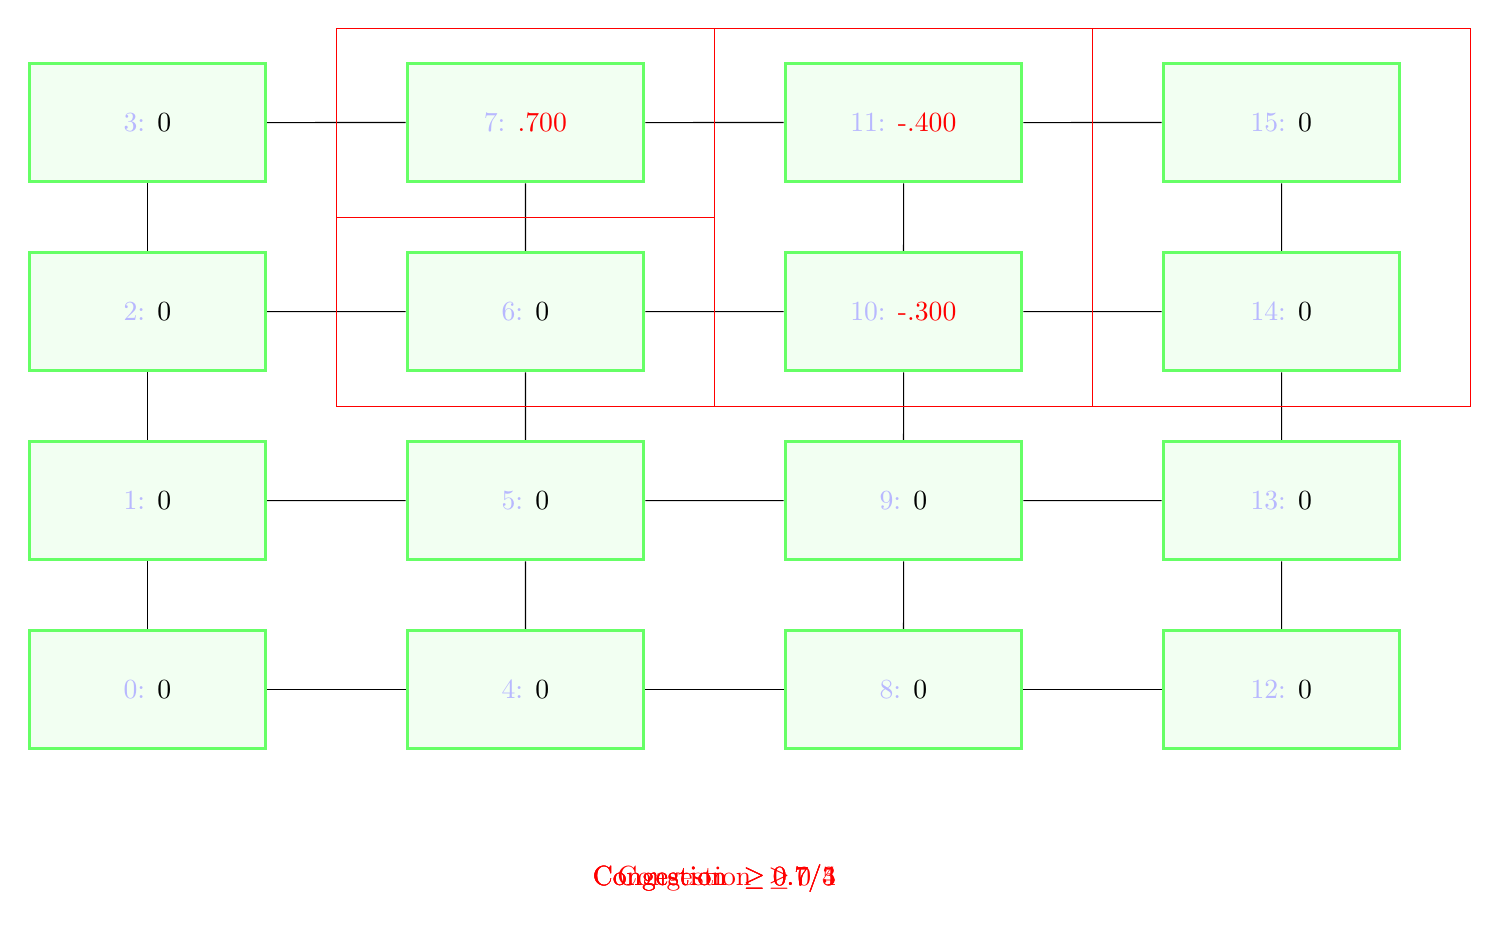
\begin{tikzpicture}[roundnode/.style={rectangle, draw=green!60, fill=green!5, very thick, minimum size=7mm, minimum width=3cm, minimum height=1.5cm}, scale=1.2]
\vspace{0.8cm}
\node<+->[roundnode] at (0.0, 0.0) (0) {\textcolor{blue!28}{0:} 0};
\node<.->[roundnode] at (0.0, 2.0) (1) {\textcolor{blue!28}{1:} 0};
\draw<.-> (1) -- (0);
\node<.->[roundnode] at (0.0, 4.0) (2) {\textcolor{blue!28}{2:} 0};
\draw<.-> (2) -- (1);
\node<.->[roundnode] at (0.0, 6.0) (3) {\textcolor{blue!28}{3:} 0};
\draw<.-> (3) -- (2);
\node<.->[roundnode] at (4.0, 0.0) (4) {\textcolor{blue!28}{4:} 0};
\draw<.-> (4) -- (0);
\node<.->[roundnode] at (4.0, 2.0) (5) {\textcolor{blue!28}{5:} 0};
\draw<.-> (5) -- (1);
\draw<.-> (5) -- (4);
\node<.->[roundnode] at (4.0, 4.0) (6) {\textcolor{blue!28}{6:} 0};
\draw<.-> (6) -- (2);
\draw<.-> (6) -- (5);
\node<.->[roundnode] at (4.0, 6.0) (7) {\textcolor{blue!28}{7:} \textcolor{red}{.700}};
\draw<.-> (7) -- (3);
\draw<.-> (7) -- (6);
\node<.->[roundnode] at (8.0, 0.0) (8) {\textcolor{blue!28}{8:} 0};
\draw<.-> (8) -- (4);
\node<.->[roundnode] at (8.0, 2.0) (9) {\textcolor{blue!28}{9:} 0};
\draw<.-> (9) -- (5);
\draw<.-> (9) -- (8);
\node<.->[roundnode] at (8.0, 4.0) (10) {\textcolor{blue!28}{10:} \textcolor{red}{-.300}};
\draw<.-> (10) -- (6);
\draw<.-> (10) -- (9);
\node<.->[roundnode] at (8.0, 6.0) (11) {\textcolor{blue!28}{11:} \textcolor{red}{-.400}};
\draw<.-> (11) -- (7);
\draw<.-> (11) -- (10);
\node<.->[roundnode] at (12.0, 0.0) (12) {\textcolor{blue!28}{12:} 0};
\draw<.-> (12) -- (8);
\node<.->[roundnode] at (12.0, 2.0) (13) {\textcolor{blue!28}{13:} 0};
\draw<.-> (13) -- (9);
\draw<.-> (13) -- (12);
\node<.->[roundnode] at (12.0, 4.0) (14) {\textcolor{blue!28}{14:} 0};
\draw<.-> (14) -- (10);
\draw<.-> (14) -- (13);
\node<.->[roundnode] at (12.0, 6.0) (15) {\textcolor{blue!28}{15:} 0};
\draw<.-> (15) -- (11);
\draw<.-> (15) -- (14);
\draw<.(5)-.(5)>[red] (2,7) -- (2,5) -- (6,5) -- (6,7) -- (2,7);
\node<.(5)-.(5)> at (6.0,-2.0) (t1) {\textcolor{red}{$\text{Congestion }\geq 0.7/3$}};
\draw<.(6)-.(6)>[red] (6,7) -- (6,3) -- (10,3) -- (10,7) -- (6,7);
\node<.(6)-.(6)> at (6.0,-2.0) (t2) {\textcolor{red}{$\text{Congestion }\geq 0.7/5$}};
\draw<.(7)-.(7)>[red] (6,7) -- (6,3) -- (14,3) -- (14,7) -- (6,7);
\node<.(7)-.(7)> at (6.0,-2.0) (t3) {\textcolor{red}{$\text{Congestion }\geq 0.7/4$}};
\draw<.(8)-.(8)>[red] (2,7) -- (2,3) -- (10,3) -- (10,7) -- (2,7);
\node<.(8)-.(8)> at (6.0,-2.0) (t4) {\textcolor{red}{$\text{Congestion }\geq 0$}};
\end{tikzpicture}
\end{center}
}
\end{frame}

\begin{frame}
\frametitle<.->{Approximator Scheme}
\begin{center}
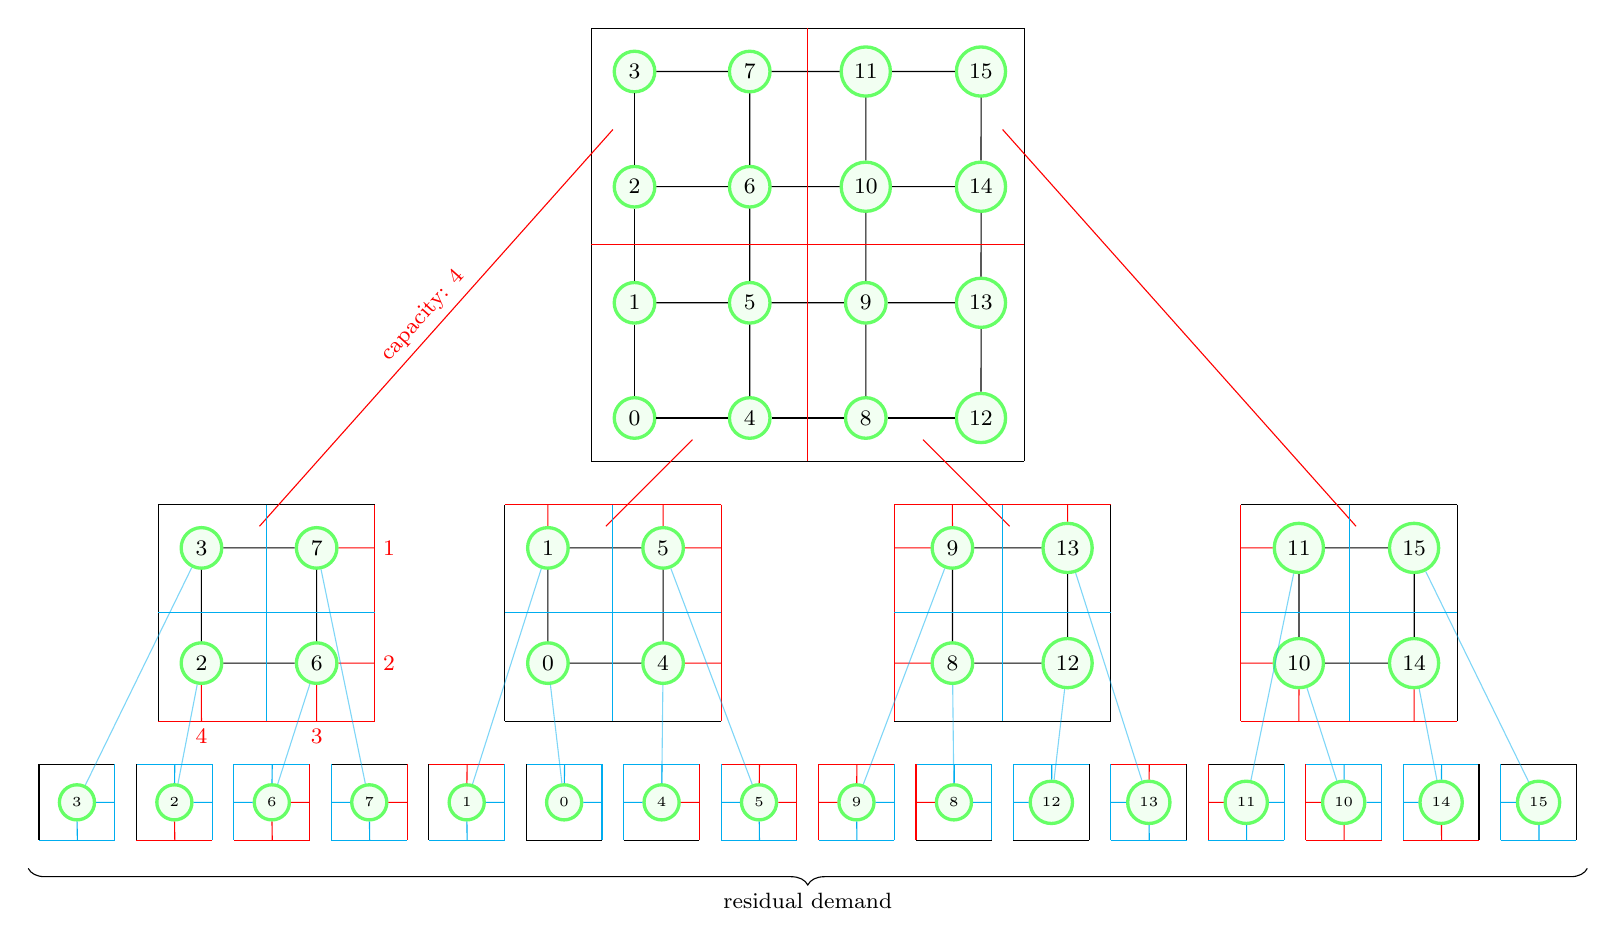
\begin{tikzpicture}[roundnode/.style={circle, draw=green!60, fill=green!5, very thick, minimum size=7mm}, scale=1.1]
\footnotesize
\node[roundnode, minimum size = .5cm] at (0.0, 0.0) (0) {\textcolor{black}{0}};
\node[roundnode, minimum size = .5cm] at (0.0, 1.33) (1) {\textcolor{black}{1}};
\draw (1) -- (0);
\node[roundnode, minimum size = .5cm] at (0.0, 2.67) (2) {\textcolor{black}{2}};
\draw (2) -- (1);
\node[roundnode, minimum size = .5cm] at (0.0, 4.0) (3) {\textcolor{black}{3}};
\draw (3) -- (2);
\node[roundnode, minimum size = .5cm] at (1.33, 0.0) (4) {\textcolor{black}{4}};
\draw (4) -- (0);
\node[roundnode, minimum size = .5cm] at (1.33, 1.33) (5) {\textcolor{black}{5}};
\draw (5) -- (1);
\draw (5) -- (4);
\node[roundnode, minimum size = .5cm] at (1.33, 2.67) (6) {\textcolor{black}{6}};
\draw (6) -- (2);
\draw (6) -- (5);
\node[roundnode, minimum size = .5cm] at (1.33, 4.0) (7) {\textcolor{black}{7}};
\draw (7) -- (3);
\draw (7) -- (6);
\node[roundnode, minimum size = .5cm] at (2.67, 0.0) (8) {\textcolor{black}{8}};
\draw (8) -- (4);
\node[roundnode, minimum size = .5cm] at (2.67, 1.33) (9) {\textcolor{black}{9}};
\draw (9) -- (5);
\draw (9) -- (8);
\node[roundnode, minimum size = .5cm] at (2.67, 2.67) (10) {\textcolor{black}{10}};
\draw (10) -- (6);
\draw (10) -- (9);
\node[roundnode, minimum size = .5cm] at (2.67, 4.0) (11) {\textcolor{black}{11}};
\draw (11) -- (7);
\draw (11) -- (10);
\node[roundnode, minimum size = .5cm] at (4.0, 0.0) (12) {\textcolor{black}{12}};
\draw (12) -- (8);
\node[roundnode, minimum size = .5cm] at (4.0, 1.33) (13) {\textcolor{black}{13}};
\draw (13) -- (9);
\draw (13) -- (12);
\node[roundnode, minimum size = .5cm] at (4.0, 2.67) (14) {\textcolor{black}{14}};
\draw (14) -- (10);
\draw (14) -- (13);
\node[roundnode, minimum size = .5cm] at (4.0, 4.0) (15) {\textcolor{black}{15}};
\draw (15) -- (11);
\draw (15) -- (14);
\draw (-0.5,-0.5) -- (-0.5,4.5);
\draw (-0.5,-0.5) -- (4.5,-0.5);
\draw (4.5,4.5) -- (-0.5,4.5);
\draw (4.5,4.5) -- (4.5,-0.5);
\draw[color=red] (-0.5,2) -- (4.5, 2);
\draw[color=red] (2,-0.5) -- (2, 4.5);
% layer 2-1
\node[roundnode, minimum size = .5cm] at (-5, -1.5) (3b) {\textcolor{black}{3}};
\node[roundnode, minimum size = .5cm] at (-5, -2.83) (2b) {\textcolor{black}{2}};
\node[roundnode, minimum size = .5cm] at (-3.67, -1.5) (7b) {\textcolor{black}{7}};
\node[roundnode, minimum size = .5cm] at (-3.67, -2.83) (6b) {\textcolor{black}{6}};
\draw (2b) -- (3b);
\draw (6b) -- (7b);
\draw (2b) -- (6b);
\draw (3b) -- (7b);
% boundaries (2-1)
\draw (-5.5,-1) -- (-3, -1);
\draw[color=red] (-3, -1) -- (-3, -3.5);
\draw[color=red] (-3,-3.5) -- (-5.5, -3.5);
\draw (-5.5,-3.5) -- (-5.5,-1);
\draw[color=red] (7b) -- (-3, -1.5) node[right]{1};
\draw[color=red] (6b) -- (-3, -2.83) node[right]{2};
\draw[color=red] (6b) -- (-3.67, -3.5) node[below]{3};
\draw[color=red] (2b) -- (-5, -3.5) node[below]{4};
% layer 2-2
\node[roundnode, minimum size = .5cm] at (-1, -1.5) (1b) {\textcolor{black}{1}};
\node[roundnode, minimum size = .5cm] at (-1, -2.83) (0b) {\textcolor{black}{0}};
\node[roundnode, minimum size = .5cm] at (0.33, -1.5) (5b) {\textcolor{black}{5}};
\node[roundnode, minimum size = .5cm] at (0.33, -2.83) (4b) {\textcolor{black}{4}};
\draw (0b) -- (1b);
\draw (4b) -- (5b);
\draw (0b) -- (4b);
\draw (1b) -- (5b);
% boundaries (2-2)
\draw[color=red] (-1.5,-1) -- (1, -1);
\draw[color=red] (1, -1) -- (1, -3.5);
\draw (1,-3.5) -- (-1.5, -3.5);
\draw (-1.5,-3.5) -- (-1.5,-1);
\draw[color=red] (1b) -- (-1,-1);
\draw[color=red] (5b) -- (0.33, -1);
\draw[color=red] (5b) -- (1, -1.5);
\draw[color=red] (4b) -- (1, -2.83);
% layer 2-3
\node[roundnode, minimum size = .5cm] at (3.67, -1.5) (9b) {\textcolor{black}{9}};
\node[roundnode, minimum size = .5cm] at (3.67, -2.83) (8b) {\textcolor{black}{8}};
\node[roundnode, minimum size = .5cm] at (5, -1.5) (13b) {\textcolor{black}{13}};
\node[roundnode, minimum size = .5cm] at (5, -2.83) (12b) {\textcolor{black}{12}};
\draw (8b) -- (9b);
\draw (12b) -- (13b);
\draw (8b) -- (12b);
\draw (9b) -- (13b);
% boundaries (2-3)
\draw[color=red] (3,-1) -- (5.5, -1);
\draw (5.5, -1) -- (5.5, -3.5);
\draw (5.5,-3.5) -- (3, -3.5);
\draw[color=red] (3,-3.5) -- (3,-1);
\draw[color=red] (9b) -- (3.67,-1);
\draw[color=red] (13b) -- (5, -1);
\draw[color=red] (9b) -- (3, -1.5);
\draw[color=red] (8b) -- (3, -2.83);
% layer 2-4
\node[roundnode, minimum size = .5cm] at (7.67, -1.5) (11b) {\textcolor{black}{11}};
\node[roundnode, minimum size = .5cm] at (7.67, -2.83) (10b) {\textcolor{black}{10}};
\node[roundnode, minimum size = .5cm] at (9, -1.5) (15b) {\textcolor{black}{15}};
\node[roundnode, minimum size = .5cm] at (9, -2.83) (14b) {\textcolor{black}{14}};
\draw (10b) -- (11b);
\draw (14b) -- (15b);
\draw (10b) -- (14b);
\draw (11b) -- (15b);
% boundaries (2-4)
\draw (7,-1) -- (9.5, -1);
\draw (9.5, -1) -- (9.5, -3.5);
\draw[color=red] (9.5,-3.5) -- (7, -3.5);
\draw[color=red] (7,-3.5) -- (7,-1);
\draw[color=red] (11b) -- (7, -1.5);
\draw[color=red] (10b) -- (7, -2.83);
\draw[color=red] (10b) -- (7.67, -3.5);
\draw[color=red] (14b) -- (9, -3.5);
% linking layers 1 + 2
\draw[color=red] (-0.25,3.33) -- (-4.33, -1.25) node[midway, sloped,above] {\textcolor{red}{capacity: $4$}};
\draw[color=red] (4.25,3.33) -- (8.33,-1.25);
\draw[color=red] (0.67,-0.25) -- (-0.33,-1.25);
\draw[color=red] (3.33,-0.25) -- (4.33,-1.25);
% seperators for layer 3
\draw[color=cyan] (-5.5,-2.25) -- (-3,-2.25);
\draw[color=cyan] (-4.25,-1) -- (-4.25, -3.5);
\draw[color=cyan] (-1.5,-2.25) -- (1,-2.25);
\draw[color=cyan] (-0.25,-1) -- (-0.25, -3.5);
\draw[color=cyan] (3,-2.25) -- (5.5,-2.25);
\draw[color=cyan] (4.25,-1) -- (4.25, -3.5);
\draw[color=cyan] (7,-2.25) -- (9.5,-2.25);
\draw[color=cyan] (8.25,-1) -- (8.25, -3.5);
% layer 3
%\foreach \x in {0, ..., 15}{\node[roundnode, minimum size=0cm] (c\x) at (\x*1.125-6.4375,-4.4375) {\tiny\x};};
\foreach [count=\xcnt] \x in {3,2,6,7,1,0,4,5,9,8,12,13,11,10,14,15}{
 \node[roundnode, minimum size=0cm] (ci\xcnt) at (\xcnt*1.125-7.5625,-4.4375) {\tiny\x};
};
% use index, not label, as variable here
%  top
%\foreach \x in {0,3,12,15}{\draw (\x*1.125-6.875,-4) -- (\x*1.125-6,-4);};
%\foreach \x in {4,7,8,11}{\draw[color=red] (\x*1.125-6.875,-4) -- (\x*1.125-6,-4);};
%\foreach \x in {1,2,5,6,9,10,13,14}{\draw[color=cyan] (\x*1.125-6.875,-4) -- (\x*1.125-6,-4);};
%  top
\foreach \x in {1,4,13,16}{\draw (\x*1.125-8,-4) -- (\x*1.125-7.125,-4);};
\foreach \x in {5,8,9,12}{
 \draw[color=red] (\x*1.125-8,-4) -- (\x*1.125-7.125,-4);
 \draw[color=red] (\x*1.125-7.5575,-4) -- (ci\x);};
\foreach \x in {2,3,6,7,10,11,14,15}{
 \draw[color=cyan] (\x*1.125-8,-4) -- (\x*1.125-7.125,-4);
 \draw[color=cyan] (\x*1.125-7.5575,-4) -- (ci\x);};
%  top / linking
%\foreach \x in {0,4,8,12}{\draw (\x*1.125-5.25, -1.5) -- (\x*1.125-6.4375,-4.4375);};
\begin{scope}[semitransparent]
 \foreach [count=\xcnt] \x in {3,2,6,7,1,0,4,5,9,8,12,13,11,10,14,15}{
  \draw[color=cyan] (\x b) -- (ci\xcnt);
 };
% \draw[color=cyan] (3b) -- (ci1) node[midway, sloped, above=2]{capacity: $2$};
% \draw[color=cyan] (1b) -- (ci5) node[midway, sloped, above=6]{capacity: $3$};
% \draw[color=cyan] (9b) -- (ci9) node[midway, sloped, above=8]{capacity: $4$};
% \draw[color=cyan] (11b) -- (ci13) node[midway, sloped, above=12]{capacity: $3$};
\end{scope}
%  left
\foreach \x in {1,2,5,6}{\draw (\x*1.125-8,-4) -- (\x*1.125-8,-4.875);};
\foreach \x in {9,10,13,14}{
 \draw[color=red] (\x*1.125-8,-4) -- (\x*1.125-8,-4.875);
 \draw[color=red] (\x*1.125-8,-4.4375) -- (ci\x);};
\foreach \x in {3,4,7,8,11,12,15,16}{
 \draw[color=cyan] (\x*1.125-8,-4) -- (\x*1.125-8,-4.875);
 \draw[color=cyan] (\x*1.125-8,-4.4375) -- (ci\x);};
%  bottom
\foreach \x in {6,7,10,11}{\draw (\x*1.125-8,-4.875) -- (\x*1.125-7.125,-4.875);};
\foreach \x in {2,3,14,15}{
 \draw[color=red] (\x*1.125-8,-4.875) -- (\x*1.125-7.125,-4.875);
 \draw[color=red] (\x*1.125-7.5575,-4.875) -- (ci\x);};
\foreach \x in {1,4,5,8,9,12,13,16}{
 \draw[color=cyan] (\x*1.125-8,-4.875) -- (\x*1.125-7.125,-4.875);
 \draw[color=cyan] (\x*1.125-7.5575,-4.875) -- (ci\x);};
%  right
\foreach \x in {11,12,15,16}{\draw (\x*1.125-7.125,-4.875) -- (\x*1.125-7.125,-4);};
\foreach \x in {3,4,7,8}{
 \draw[color=red] (\x*1.125-7.125,-4.875) -- (\x*1.125-7.125,-4);
 \draw[color=red] (\x*1.125-7.125,-4.4375) -- (ci\x);};
\foreach \x in {1,2,5,6,9,10,13,14}{
 \draw[color=cyan] (\x*1.125-7.125,-4.875) -- (\x*1.125-7.125,-4);
 \draw[color=cyan] (\x*1.125-7.125,-4.4375) -- (ci\x);};

% demand
 \draw[decorate, decoration = {brace, amplitude=6pt}] (11,-5.2) -- (-7,-5.2) node[midway, below=6pt]{residual demand};
\end{tikzpicture}
\end{center}
\end{frame}

\begin{frame}
\frametitle<.->{$\alpha$-Congestion Approximator}
Definition:
\begin{align*}
\Vert Rb\Vert_\infty\leq \text{opt}(b)\leq \alpha\Vert Rb\Vert_\infty,&\text{  ~~for all demands $b$}
\end{align*}
opt$(b)$: Minimum Congestion for $b$ \pause

Equivalent iff $Rb\neq 0$:
\begin{align*}
1\leq \frac{\text{opt}(b)}{\Vert Rb\Vert_\infty}\leq \alpha ,&\text{  ~~for all demands $b$}
\end{align*}
\end{frame}


\begin{frame}
\frametitle<.->{Potential Function}
\begin{align*}
\Phi (f)&\coloneqq \left\Vert C^{-1}f\right\Vert_\infty+2\alpha\left\Vert R(b-Bf)\right\Vert_\infty\\
\phi(f)&\coloneqq lmax\left(C^{-1}f\right)+lmax\left(2\alpha\cdot R(b-Bf)\right)\\
\nabla\phi(f)&=\left(C^{-1}\right)^T\cdot \nabla lmax\left(C^{-1}f\right)-2\alpha\cdot B^TR^T\cdot\nabla lmax(2\alpha\cdot R(b-Bf))\\\\
lmax(\vec{x})&\coloneqq ln\left(\sum_ie^{x_i}+e^{-x_i}\right)\\
\left(\nabla lmax(\vec{x})\right)_j&=\frac{e^{x_j}-e^{-x_j}}{\sum_ie^{x_i}+e^{-x_i}}
\end{align*}
\end{frame}

\begin{frame}
\frametitle<.->{Potential Function}
\begin{center}
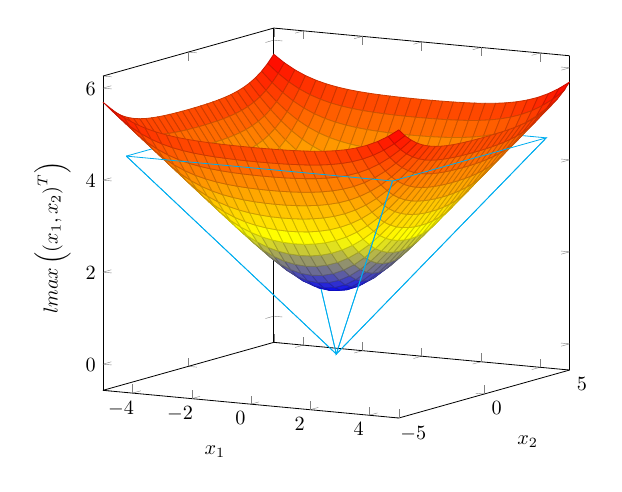
\begin{tikzpicture}[declare function={f(\x,\y)=max(\x,\y,-1*\x,-1*\y);}, scale=0.73]
\begin{axis}[
  view = {30}{10},
  samples = 29,
  xlabel=$x_1$,
  ylabel=$x_2$,
  zlabel={$lmax\left(\left(x_1,x_2\right)^T\right)$},
  width = 0.8*\linewidth,
]
\addplot3 [mark=none,cyan] coordinates{ (-4.5,-4.5,4.5) (0,0,0) (-4.5,4.5,4.5) (-4.5,-4.5,4.5)};
\addplot3 [mark=none,cyan] coordinates{ (4.5,4.5,4.5) (0,0,0) (-4.5,4.5,4.5) (4.5,4.5,4.5)};
\addplot3 [surf] {ln(e^x+e^(-x)+e^y+e^(-y))};
\addplot3 [mark=none,cyan] coordinates{ (-4.5,-4.5,4.5) (0,0,0) (4.5,-4.5,4.5) (-4.5,-4.5,4.5)};
\addplot3 [mark=none,cyan] coordinates{ (4.5,-4.5,4.5) (0,0,0) (4.5,4.5,4.5) (4.5,-4.5,4.5)};
\end{axis}
\end{tikzpicture}
\end{center}
\end{frame}

\begin{frame}
\frametitle<.->{Congestion Approximator}

\begin{center}
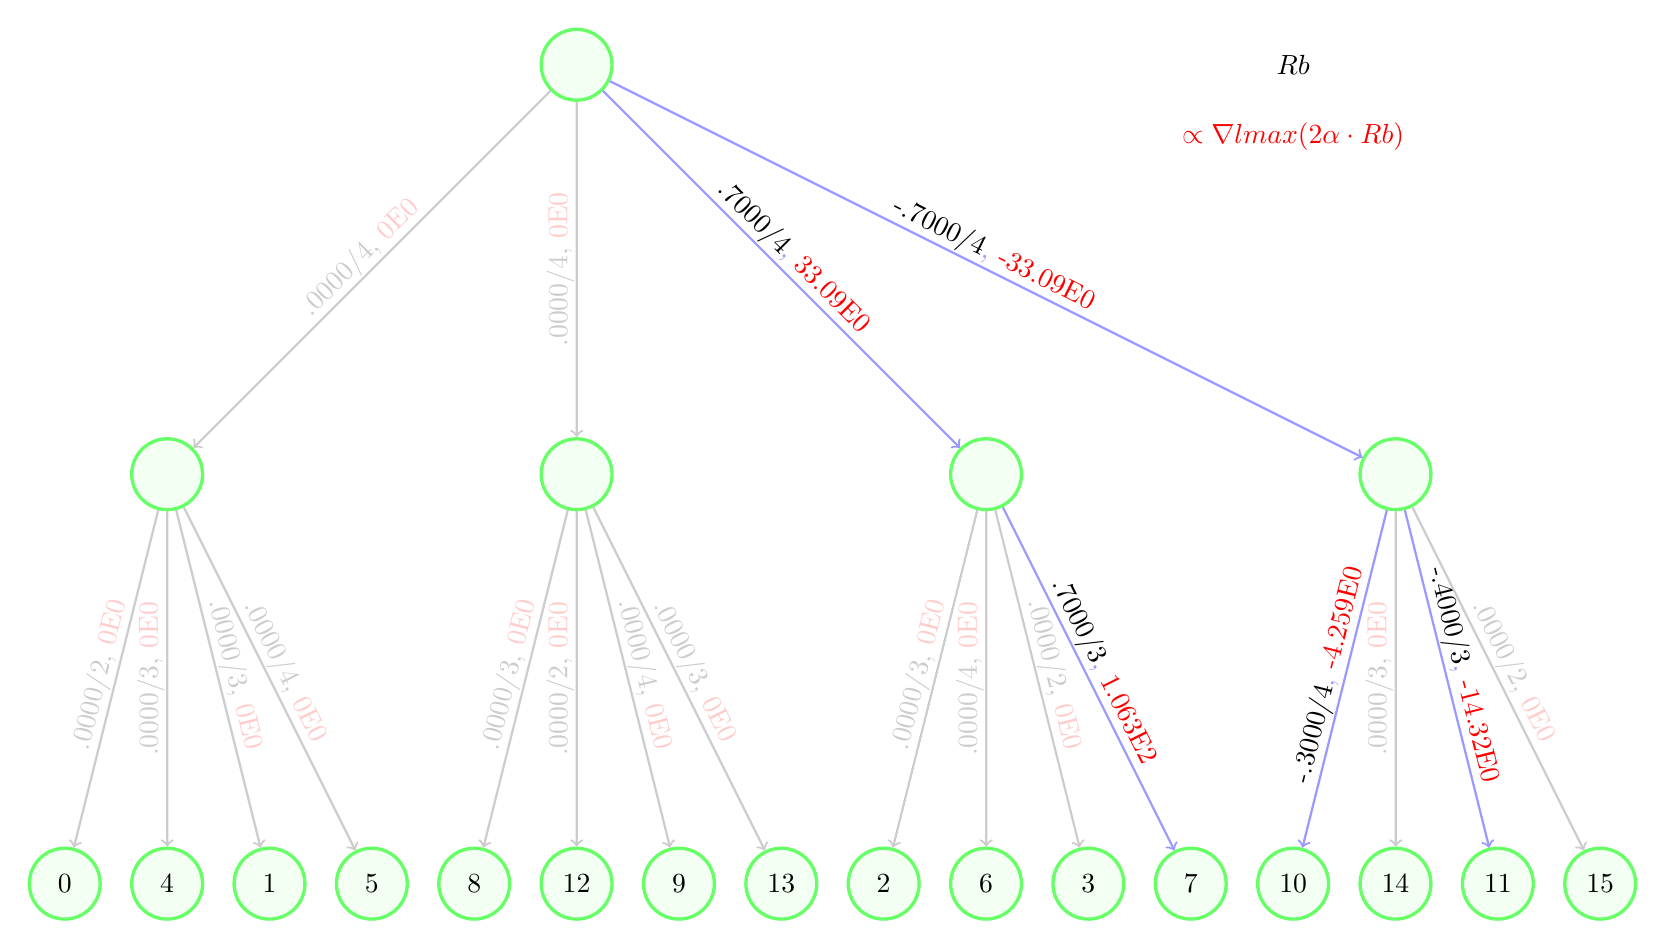
\begin{tikzpicture}[roundnode/.style={circle, draw=green!60, fill=green!5, very thick, minimum size=7mm}, scale=1.3]
%\hspace{-3cm}
\node[roundnode, minimum size = 0.9cm] at (8.0, 8) (0h8) {};
\node[roundnode, minimum size = 0.9cm] at (4.0, 4) (2h4) {};
\node[roundnode, minimum size = 0.9cm] at (3.0, 0) (2h0) {0};
\draw[thick, ->, color=black!20] (2h4) -- (2h0) node[sloped,midway,above=-0.1cm] {\textcolor{black!20}{.0000/2}, \textcolor{red!20}{0E0}};
\node[roundnode, minimum size = 0.9cm] at (4.0, 0) (3h0) {4};
\draw[thick, ->, color=black!20] (2h4) -- (3h0) node[sloped,midway,above=-0.1cm] {\textcolor{black!20}{.0000/3}, \textcolor{red!20}{0E0}};
\node[roundnode, minimum size = 0.9cm] at (5.0, 0) (4h0) {1};
\draw[thick, ->, color=black!20] (2h4) -- (4h0) node[sloped,midway,above=-0.1cm] {\textcolor{black!20}{.0000/3}, \textcolor{red!20}{0E0}};
\node[roundnode, minimum size = 0.9cm] at (6.0, 0) (5h0) {5};
\draw[thick, ->, color=black!20] (2h4) -- (5h0) node[sloped,midway,above=-0.1cm] {\textcolor{black!20}{.0000/4}, \textcolor{red!20}{0E0}};
\draw[thick, ->, color=black!20] (0h8) -- (2h4) node[sloped,midway,above=-0.1cm] {\textcolor{black!20}{.0000/4}, \textcolor{red!20}{0E0}};
\node[roundnode, minimum size = 0.9cm] at (8.0, 4) (6h4) {};
\node[roundnode, minimum size = 0.9cm] at (7.0, 0) (6h0) {8};
\draw[thick, ->, color=black!20] (6h4) -- (6h0) node[sloped,midway,above=-0.1cm] {\textcolor{black!20}{.0000/3}, \textcolor{red!20}{0E0}};
\node[roundnode, minimum size = 0.9cm] at (8.0, 0) (7h0) {12};
\draw[thick, ->, color=black!20] (6h4) -- (7h0) node[sloped,midway,above=-0.1cm] {\textcolor{black!20}{.0000/2}, \textcolor{red!20}{0E0}};
\node[roundnode, minimum size = 0.9cm] at (9.0, 0) (8h0) {9};
\draw[thick, ->, color=black!20] (6h4) -- (8h0) node[sloped,midway,above=-0.1cm] {\textcolor{black!20}{.0000/4}, \textcolor{red!20}{0E0}};
\node[roundnode, minimum size = 0.9cm] at (10.0, 0) (9h0) {13};
\draw[thick, ->, color=black!20] (6h4) -- (9h0) node[sloped,midway,above=-0.1cm] {\textcolor{black!20}{.0000/3}, \textcolor{red!20}{0E0}};
\draw[thick, ->, color=black!20] (0h8) -- (6h4) node[sloped,midway,above=-0.1cm] {\textcolor{black!20}{.0000/4}, \textcolor{red!20}{0E0}};
\node[roundnode, minimum size = 0.9cm] at (12.0, 4) (10h4) {};
\node[roundnode, minimum size = 0.9cm] at (11.0, 0) (10h0) {2};
\draw[thick, ->, color=black!20] (10h4) -- (10h0) node[sloped,midway,above=-0.1cm] {\textcolor{black!20}{.0000/3}, \textcolor{red!20}{0E0}};
\node[roundnode, minimum size = 0.9cm] at (12.0, 0) (11h0) {6};
\draw[thick, ->, color=black!20] (10h4) -- (11h0) node[sloped,midway,above=-0.1cm] {\textcolor{black!20}{.0000/4}, \textcolor{red!20}{0E0}};
\node[roundnode, minimum size = 0.9cm] at (13.0, 0) (12h0) {3};
\draw[thick, ->, color=black!20] (10h4) -- (12h0) node[sloped,midway,above=-0.1cm] {\textcolor{black!20}{.0000/2}, \textcolor{red!20}{0E0}};
\node[roundnode, minimum size = 0.9cm] at (14.0, 0) (13h0) {7};
\draw[thick, ->, color=blue!40] (10h4) -- (13h0) node[sloped,midway,above=-0.1cm] {\textcolor{black}{.7000/3}, \textcolor{red}{1.063E2}};
\draw[thick, ->, color=blue!40] (0h8) -- (10h4) node[sloped,midway,above=-0.1cm] {\textcolor{black}{.7000/4}, \textcolor{red}{33.09E0}};
\node[roundnode, minimum size = 0.9cm] at (16.0, 4) (14h4) {};
\node[roundnode, minimum size = 0.9cm] at (15.0, 0) (14h0) {10};
\draw[thick, ->, color=blue!40] (14h4) -- (14h0) node[sloped,midway,above=-0.1cm] {\textcolor{black}{-.3000/4}, \textcolor{red}{-4.259E0}};
\node[roundnode, minimum size = 0.9cm] at (16.0, 0) (15h0) {14};
\draw[thick, ->, color=black!20] (14h4) -- (15h0) node[sloped,midway,above=-0.1cm] {\textcolor{black!20}{.0000/3}, \textcolor{red!20}{0E0}};
\node[roundnode, minimum size = 0.9cm] at (17.0, 0) (16h0) {11};
\draw[thick, ->, color=blue!40] (14h4) -- (16h0) node[sloped,midway,above=-0.1cm] {\textcolor{black}{-.4000/3}, \textcolor{red}{-14.32E0}};
\node[roundnode, minimum size = 0.9cm] at (18.0, 0) (17h0) {15};
\draw[thick, ->, color=black!20] (14h4) -- (17h0) node[sloped,midway,above=-0.1cm] {\textcolor{black!20}{.0000/2}, \textcolor{red!20}{0E0}};
\draw[thick, ->, color=blue!40] (0h8) -- (14h4) node[sloped,midway,above=-0.1cm] {\textcolor{black}{-.7000/4}, \textcolor{red}{-33.09E0}};

\node[black] at (15.0,8) {$Rb$};
\node[red] at (15.0,7.3) {$\propto\nabla lmax(2\alpha\cdot Rb)$};
\end{tikzpicture}
\end{center}
\end{frame}

\begin{frame}
\frametitle<+->{Grid Graphs}
\begin{itemize}
\item<+-> Undirected
\item<+-> Unit-Capacity
\item<+-> Multi-Dimensional
\item<+-> $\rightarrow$ can be defined via dimensional node count vector $(n_1,...,n_d)$
\end{itemize}
\end{frame}

\begin{frame}
\frametitle<.->{Grid Graphs}
Node count:
\begin{align*}
n&=\prod_{i=1}^dn_i
\end{align*}
Edge count:
\begin{align*}
m&=\left(\sum_{i=1}^d\frac{n_i-1}{n_i}\right)\cdot n\\\\
&\rightarrow m\in\Theta(d\cdot n)
\end{align*}
\end{frame}

\begin{frame}
\frametitle<.->{Grid Graphs}
Capacity of hypercube cut $([a_1,b_1], ...,[a_d,b_d])$:
\begin{align*}
\sum_{i=1}^d\left((\overline{\delta}_{a_i,0}+\overline{\delta}_{b_i,n_i-1})\cdot \prod_{j=1,j\neq i}^d(b_j-a_j+1)\right)
\end{align*}
with $\overline{\delta}_{x,y}=1-\delta_{x,y}$ (Kronecker-Delta)
\end{frame}


\begin{frame}
\frametitle<.->{Algorithm}
\hspace{2cm}
\begin{algorithm}[H]
%\caption{\texttt{AlmostRoute} algorithm from \cite{nmfnlt}.}\label{alg_almostroute}
\begin{algorithmic}[1]
\Procedure{CompleteRoute}{$b$, $\varepsilon$}
\State $r\gets b$
\State $(f_0,S_0)\gets \texttt{AlmostRoute}(r,\varepsilon)$
\For{$i\gets 1,\log_2(2m)$}
  \State $r\gets r-Bf_{i-1}$
  \State $(f_i,S_i)\gets \texttt{AlmostRoute}(r, 1/2)$
\EndFor
\State $r\gets r-Bf_i$\Comment{Assuming $i=log(2m)$ after the loop.}
\State $f_{i+1}\gets \texttt{GridMST.route}(r)$
\State \Return $\sum_{j=0}^{i+1}f_j$
\EndProcedure
\end{algorithmic}
\end{algorithm}
\end{frame}

\begin{frame}
\frametitle<.->{Algorithm}
\hspace{2cm}
\begin{algorithm}[H]
%\caption{\texttt{AlmostRoute} algorithm from \cite{nmfnlt}.}\label{alg_almostroute}
\begin{algorithmic}[1]
\Procedure{AlmostRoute}{$b$, $\varepsilon$}
\Repeat
  \While{$\phi(f)<16\varepsilon^{-1}\log(n)$}
    \State $f\gets \mathsmaller{\frac{17}{16}}\cdot f$
    \State $b\gets \mathsmaller{\frac{17}{16}}\cdot b$
  \EndWhile
  \State $\delta\gets \Vert C\nabla \phi(f)\Vert_1$
  \If{$\delta\geq \varepsilon/4$}
    \State $f_e\gets f_e-\frac{\delta}{1+4\alpha^2}\text{sgn}(\nabla \phi(f)_e)c_e$
  \EndIf
\Until{$\delta<\varepsilon/4$}
\State \Return $f$, $\nabla\phi(f)$
\EndProcedure
\end{algorithmic}
\end{algorithm}
\end{frame}

\begin{frame}
\frametitle<.->{Maximal Spanning Tree}
\vspace{1cm}
\begin{center}
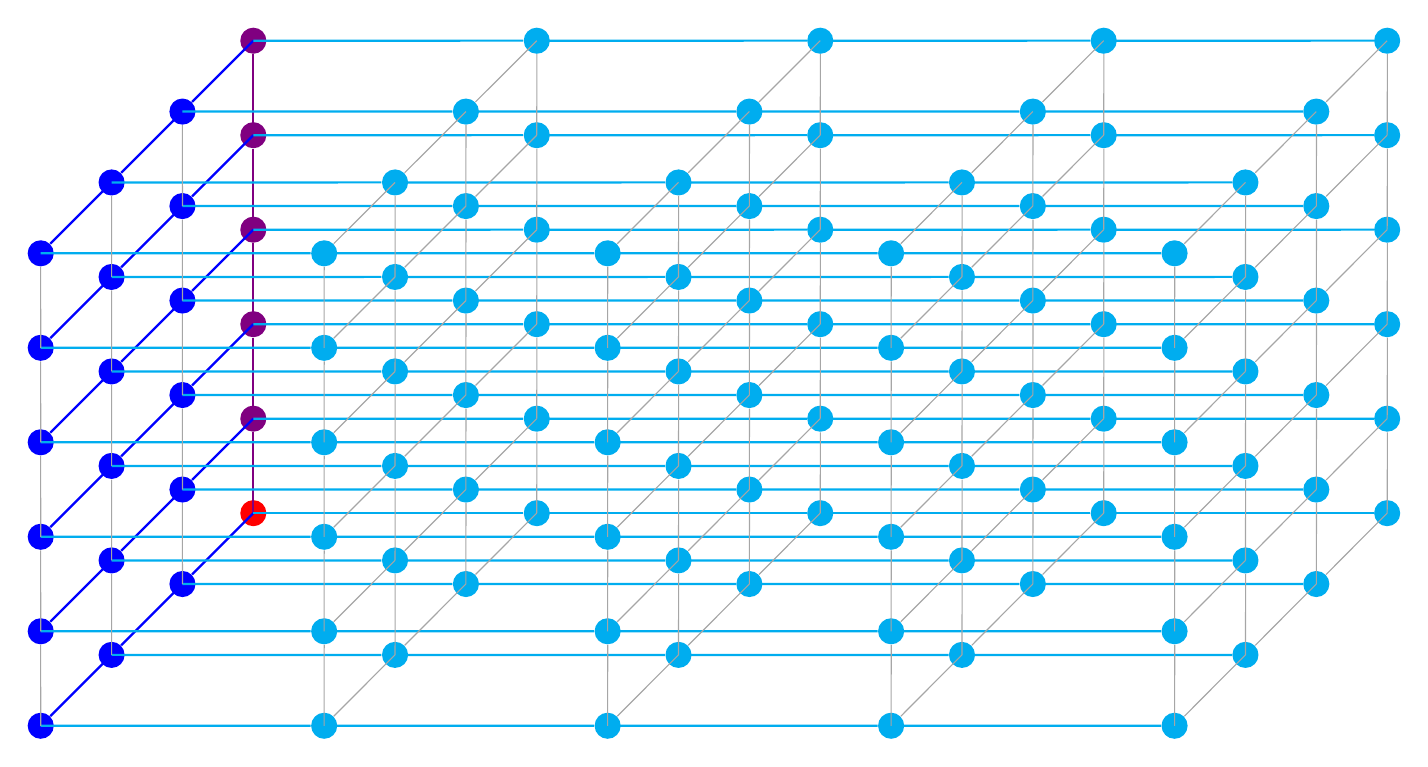
\begin{tikzpicture}[scale=1.2]
\node[circle,fill=red] at (0,0) {};
\foreach \x in {1,2,3,4,5}{
  \node[circle,fill=violet] at (0,\x) (x-0-y-0-z-\x) {};
  \draw[color=violet,thick] (x-0-y-0-z-\x) -- (0,\x-1);
};
\foreach \x in {1,2,3}{
  \foreach \y in {0,1,2,3,4,5}{
    \node[circle,fill=blue] at (-\x*0.75,-\x*0.75+\y*1) (x-0-y-\x-z-\y) {};
    \draw[color=blue,thick] (x-0-y-\x-z-\y) -- (-\x*0.75+0.75,-\x*0.75+0.75+\y*1);
  };
};
\foreach \x in {1,2,3,4}{
  \foreach \y in {0,1,2,3}{
    \foreach \z in {0,1,2,3,4,5}{
      \node[circle,fill=cyan] at (3*\x-\y*0.75,-\y*0.75+\z*1) (x-\x-y-\y-z-\z) {};
      \draw[color=cyan,thick] (x-\x-y-\y-z-\z) -- (3*\x-3-\y*0.75,-\y*0.75+\z*1);
    };
  };
};
\foreach \x in {1,2,3,4}{
  \foreach \y in {1,2,3}{
    \foreach \z in {0,1,2,3,4,5}{
      \draw[color=gray!70] (x-\x-y-\y-z-\z) -- (3*\x+0.75-\y*0.75,-\y*0.75+0.75+\z*1);
    };
  };
};
\foreach \x in {0,1,2,3,4}{
  \foreach \y in {1,2,3}{
    \foreach \z in {1,2,3,4,5}{
      \draw[color=gray!70] (x-\x-y-\y-z-\z) -- (3*\x-\y*0.75,-\y*0.75-1+\z*1);
    };
  };
};
\foreach \x in {1,2,3,4}{
  \foreach \y in {0}{
    \foreach \z in {1,2,3,4,5}{
      \draw[color=gray!70] (x-\x-y-\y-z-\z) -- (3*\x-\y*0.75,-\y*0.75-1+\z*1);
    };
  };
};
\end{tikzpicture}
\end{center}
\end{frame}

\begin{frame}
\frametitle<.->{MST Routing}
\begin{algorithm}[H]
\footnotesize
\caption{Routing Demand $b$ through a (Maximal) Spanning Tree of Grid Graph $G$}\label{alg_mst}
\begin{algorithmic}[1]
\Procedure{RouteMST}{GridGraph $G$, GridDemand $b$}
\State $f\gets 0$
\State $r\gets b$\Comment{Residual demand}
\State $(n_1,...,n_d)\gets G.nodesPerDimension$
\For{$i\gets 1,d$}
    \For{$j\gets 1,i-1$}\algorithmiccomment{Set $v_{start}$ and $v_{end}$ properly}
        \State $\left(v_{start}\right)_j\gets 0$
        \State $\left(v_{end}\right)_j\gets 0$
    \EndFor
    \State $\left(v_{start}\right)_i\gets n_i-1$
    \State $\left(v_{end}\right)_i\gets 1$
    \For{$j\gets i+1,d$}
        \State $\left(v_{start}\right)_j\gets n_j-1$
        \State $\left(v_{end}\right)_j\gets 0$
    \EndFor
    \For{$v\gets v_{start},v_{end}$}%\algorithmiccomment{\parbox[t]{.6\linewidth}{Consecutively eliminate leaves along this dimension. Iteration is valid iff for each vertex pair $v_1$ and $v_2$ with $\left(v_1\right)_j=\left(v_2\right)_j$ for $j\neq i$ and $\left(v_1\right)_i>\left(v_2\right)_i$, $v_1$ will be eliminated before $v_2$.}}
        \State $u\gets v$
        \State $u_i\gets v_i-1$
        \State $e\gets (u,v)$
        \State $f_e\gets r_v$\Comment{\parbox[t]{.6\linewidth}{$r_v$: Residual demand of leaf $v$. Every iterated $v$ is a leaf iff the iteration is valid.}}
        \State $r_u\gets r_u+r_v$
        \State $r_v\gets 0$
    \EndFor
\EndFor
\State \Return $f$
\EndProcedure
\end{algorithmic}
\end{algorithm}
\end{frame}

\begin{frame}
\frametitle<.->{MST Routing}
\vspace{5mm}
\begin{algorithm}[H]
\caption{Simplified Version}
\begin{algorithmic}[1]
\Procedure{RouteMST2}{GridGraph $G$, GridDemand $b$}
\State $f\gets 0$
\State $r\gets b$\Comment{Residual demand}
\State $i\gets 1$
\For{$k\gets n-1,1$}
    \State $\vec{v}\gets \texttt{toVector}(k)$
    \While{$\vec{v}_i=0$}
        \State $i\gets i+1$
    \EndWhile
    \State $\vec{v}_i\gets \vec{v}_i-1$
    \State $u\gets \texttt{toIndex}(\vec{v})$
    \State $e\gets (u,k)$
    \State $f_e\gets r_k$
    \State $r_u\gets r_u+r_k$
    \State $r_k\gets 0$
\EndFor
\State \Return $f$
\EndProcedure
\end{algorithmic}
\end{algorithm}
\end{frame}

\begin{frame}
\frametitle<+->{Implementation}
\begin{itemize}
\item<+-> Basic DS \& Algorithm(s)
\item<+-> Step Size Optimization
\item<+-> Empiric Search for $\alpha$
\end{itemize}
\end{frame}

\begin{frame}
\frametitle<+->{Step Size Optimization}
\begin{itemize}
\item<+-> Default: $f_i\gets f_i-s_i$
\item<+-> Approach: $f_i\gets f_i-h\cdot s_i$
\end{itemize}
\onslide<+-.(1)>{
\begin{align*}
\frac{\vartheta}{\vartheta h}\phi(f-h\cdot s)&=(-C^{-1}s)^T\cdot \nabla lmax\left(C^{-1}\cdot (f-h\cdot s)\right)+(2\alpha RBs)^T\cdot \nabla lmax\left(2\alpha R(b-B(f-h\cdot s))\right)
\end{align*}
}
\end{frame}


\begin{frame}
\frametitle<.->{Static Optimization}
\includegraphics<1>[width=0.98\linewidth, height=12cm]{PicRes/Iter-eps01-d1.png}
\includegraphics<2>[width=0.98\linewidth, height=12cm]{PicRes/Iter-eps001-d1.png}
\includegraphics<3>[width=0.98\linewidth, height=12cm]{PicRes/Iter-eps01-d2.png}
\end{frame}


\begin{frame}
\frametitle<.->{$\phi(f-h\cdot s)$}
\alt<1>{
\includegraphics[width=0.48\linewidth, height=6cm]{PicRes/optstep1.png} 
\includegraphics[width=0.48\linewidth, height=6cm]{PicRes/optstep2.png} 
\includegraphics[width=0.48\linewidth, height=6cm]{PicRes/optstep3.png}
\pause 
}{
\includegraphics[width=0.48\linewidth, height=6cm]{PicRes/optstep3ref1.png}  
\includegraphics[width=0.48\linewidth, height=6cm]{PicRes/optstep3diff.png}
\includegraphics[width=0.48\linewidth, height=6cm]{PicRes/optstep3ref2.png} 
\includegraphics[width=0.48\linewidth, height=6cm]{PicRes/optstep3diffref.png} 
}
\end{frame}

\begin{frame}
\frametitle<.->{Line Search}
\begin{figure}
\subfigure{
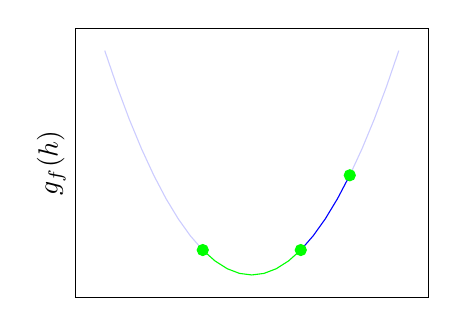
\begin{tikzpicture}
  \begin{axis}[
      domain=-3:3,
      ticks=none,
      %axis x line=bottom,
      %axis y line=left,
      %xlabel = $h$,
      ylabel = $g_f(h)$,
      width = 0.5 \textwidth,
      height = 5cm,
    ]
    \addplot[green, no marks, restrict x to domain=-1:1] {0.2*x^2+1};
    \addplot[blue, no marks, restrict x to domain=1:2] {0.2*x^2+1};
    \addplot[blue!20, no marks, restrict x to domain=-3:-1] {0.2*x^2+1};
    \addplot[blue!20, no marks, restrict x to domain=2:3] {0.2*x^2+1};
    \addplot[only marks, green, samples at={-1,1,2}]{0.2*x^2+1};
  \end{axis}
\end{tikzpicture}\label{ex_ls1}}%
\subfigure{
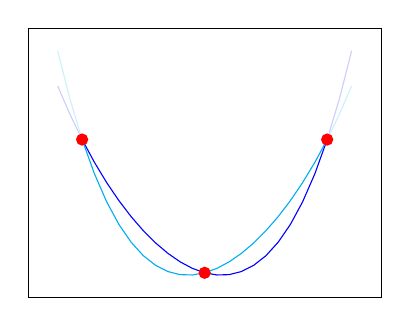
\begin{tikzpicture}
  \begin{axis}[
      domain=-1.2:1.2,
      ticks=none,
      %axis x line=bottom,
      %axis y line=left,
      %xlabel = $h$,
      %ylabel = $g_f(h)$,
      width = 0.5 \textwidth,
      height = 5cm,
    ]
    \addplot[blue!20, no marks, restrict x to domain=-1.2:-1] {0.15*x^4+0.25*x^3+0.85*x^2-0.25*x};
    \addplot[cyan!20, no marks, restrict x to domain=-1.2:-1] {0.15*x^4-0.25*x^3+0.85*x^2+0.25*x};
    \addplot[blue, no marks, restrict x to domain=-1:1] {0.15*x^4+0.25*x^3+0.85*x^2-0.25*x};
    \addplot[cyan, no marks, restrict x to domain=-1:1] {0.15*x^4-0.25*x^3+0.85*x^2+0.25*x};
    \addplot[blue!20, no marks, restrict x to domain=1:1.2] {0.15*x^4+0.25*x^3+0.85*x^2-0.25*x};
    \addplot[cyan!20, no marks, restrict x to domain=1:1.2] {0.15*x^4-0.25*x^3+0.85*x^2+0.25*x};
    \addplot[only marks, red, samples at={-1,0,1}]{0.15*x^4+0.25*x^3+0.85*x^2-0.25*x};
  \end{axis}
\end{tikzpicture}\label{ex_ls2}}\\
\subfigure{
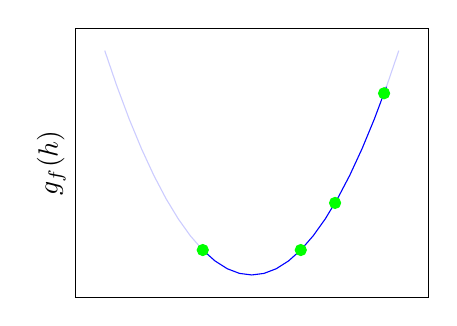
\begin{tikzpicture}
  \begin{axis}[
      domain=-3:3,
      ticks=none,
      %axis x line=bottom,
      %axis y line=left,
      %xlabel = $h$,
      ylabel = $g_f(h)$,
      width = 0.5 \textwidth,
      height = 5cm,
    ]
    \addplot[blue, no marks, restrict x to domain=-1:2.8] {0.2*x^2+1};
    \addplot[blue!20, no marks, restrict x to domain=-3:-1] {0.2*x^2+1};
    \addplot[blue!20, no marks, restrict x to domain=2.7:3] {0.2*x^2+1};
    \addplot[only marks, green, samples at={-1,1,1.7,2.7}]{0.2*x^2+1};
  \end{axis}
\end{tikzpicture}\label{ex_ls3}}%
\subfigure{
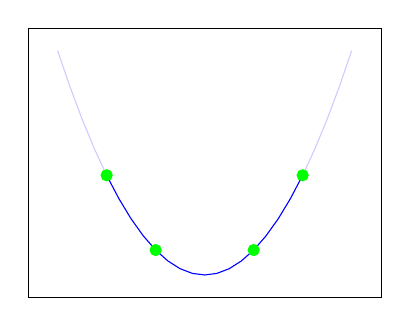
\begin{tikzpicture}
  \begin{axis}[
      domain=-3:3,
      ticks=none,
      %axis x line=bottom,
      %axis y line=left,
      %xlabel = $h$,
      %ylabel = $g_f(h)$,
      width = 0.5 \textwidth,
      height = 5cm,
    ]
    \addplot[blue, no marks, restrict x to domain=-2:2] {0.2*x^2+1};
    \addplot[blue!20, no marks, restrict x to domain=-3:-2] {0.2*x^2+1};
    \addplot[blue!20, no marks, restrict x to domain=2:3] {0.2*x^2+1};
    \addplot[only marks, green, samples at={-2,-1,1,2}]{0.2*x^2+1};
  \end{axis}
\end{tikzpicture}\label{ex_ls4}}\\
\subfigure{
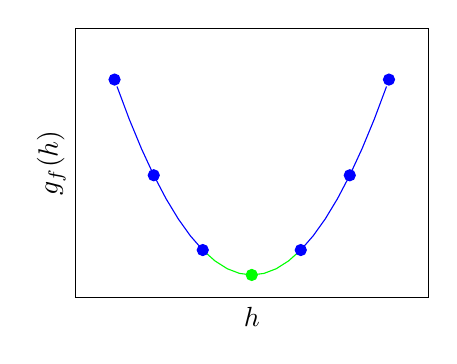
\begin{tikzpicture}
  \begin{axis}[
      domain=-3:3,
      ticks=none,
      %axis x line=bottom,
      %axis y line=left,
      xlabel = $h$,
      ylabel = $g_f(h)$,
      width = 0.5 \textwidth,
      height = 5cm,
    ]
    \addplot[blue!20, no marks, restrict x to domain=-3:-2.8] {0.2*x^2+1};
    \addplot[blue!20, no marks, restrict x to domain=2.8:3] {0.2*x^2+1};
    \addplot[blue, no marks, restrict x to domain=-2.8:-1] {0.2*x^2+1};
    \addplot[blue, no marks, restrict x to domain=1:2.8] {0.2*x^2+1};
    \addplot[green, no marks, restrict x to domain=-1:1] {0.2*x^2+1};
    \addplot[only marks, blue, samples at={-2.8,-2,-1,1,2,2.8}]{0.2*x^2+1};
    \addplot[mark=*,green] coordinates {(0,1)};
  \end{axis}
\end{tikzpicture}\vspace{0.2cm}
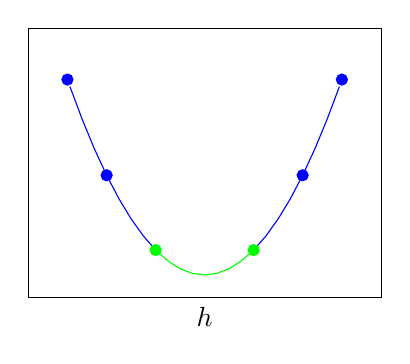
\begin{tikzpicture}
  \begin{axis}[
      domain=-3:3,
      ticks=none,
      %axis x line=bottom,
      %axis y line=left,
      xlabel = $h$,
      %ylabel = $g_f(h)$,
      width = 0.5 \textwidth,
      height = 5cm,
    ]
    \addplot[blue!20, no marks, restrict x to domain=-3:-2.8] {0.2*x^2+1};
    \addplot[blue!20, no marks, restrict x to domain=2.8:3] {0.2*x^2+1};
    \addplot[blue, no marks, restrict x to domain=-2.8:-1] {0.2*x^2+1};
    \addplot[blue, no marks, restrict x to domain=1:2.8] {0.2*x^2+1};
    \addplot[green, no marks, restrict x to domain=-1:1] {0.2*x^2+1};
    \addplot[only marks, blue, samples at={-2.8,-2,2,2.8}]{0.2*x^2+1};
    \addplot[only marks, green, samples at={-1,1}]{0.2*x^2+1};
  \end{axis}
\end{tikzpicture}
\label{ex_ls5}}
\end{figure}
\end{frame}

\begin{frame}
\frametitle<.->{Golden Section Search}
\vspace{2cm}
\begin{tikzpicture}
  \begin{axis}[
      domain=-3:3,
      ticks=none,
      %axis x line=bottom,
      %axis y line=left,
      xlabel = $h$,
      ylabel = $g_f(h)$,
      width = 0.9 \textwidth,
      height = 9cm,
    ]
    %\addplot[blue!20, no marks, restrict x to domain=-3:-2.8] {0.2*x^2+1};
    %\addplot[blue!20, no marks, restrict x to domain=2.8:3] {0.2*x^2+1};
    \addplot[blue, no marks, restrict x to domain=-2.8:-0.266,samples=31] {0.2*x^2+1};
    \addplot[blue, no marks, restrict x to domain=2.6:2.8,samples=21] {0.2*x^2+1};
    \addplot[green, no marks, restrict x to domain=-0.466:2.6, samples=71] {0.2*x^2+1};
    \addplot[only marks, red, samples at={1.467}] {0.2*x^2+1};
    %\addplot[only marks, blue, samples at={-2.8,-2,2,2.8}]{0.2*x^2+1};
    \addplot[only marks, black, samples at={-2.2,-0.366,0.766,2.6}]{0.2*x^2+1};
    \addplot[black, no marks, restrict x to domain=0.766:2.6,samples=91] {0.8};
    \addplot[black, no marks, restrict x to domain=-2.2:2.6, samples=101] {0.7};
    \addplot[red, no marks, restrict x to domain=-0.366:0.766,samples=91] {0.5};
    \addplot[red, no marks, restrict x to domain=-0.366:2.6,samples=101] {0.4};
  \end{axis}
  %\draw[red] (9,1) -- (10,2);
\end{tikzpicture}
\end{frame}

\begin{frame}
\frametitle<.->{Dynamic Optimization Results}
%\alt<1>{

\includegraphics<1>[width=0.95\linewidth, height=6cm]{PicRes/Iter-GSS-eps01-d1.png} 
\includegraphics<1>[width=0.95\linewidth, height=6cm]{PicRes/Times-GSS-eps01-d1.png} 
%\pause
%}{
%\alt<2>{
\includegraphics<2>[width=0.95\linewidth, height=6cm]{PicRes/Iter-GSS-eps001-d1.png} 
\includegraphics<2>[width=0.95\linewidth, height=6cm]{PicRes/Times-GSS-eps001-d1.png} 
%\pause
%}{
\includegraphics<3>[width=0.95\linewidth, height=6cm]{PicRes/Iter-GSS-eps001-d2.png}
\includegraphics<3>[width=0.95\linewidth, height=6cm]{PicRes/Times-GSS-eps001-d2.png} 
%}}
\end{frame}

\begin{frame}
\frametitle<+->{Empiric Search for $\alpha$}
\begin{itemize}
\item<+-> Random Sampling for 1D grid graphs
\item<+-> 1D-sampling usable in higher dimensions
\item<+-> Randomized Cut with Maximum Congestion
\item<+-> Pre-Calculating Optimal Maximum Congestion
\end{itemize}
\end{frame}

\begin{frame}
\frametitle<.->{1D-Sampling for $\alpha$}
%\includegraphics<1>[width=0.98\linewidth, height=3cm]{PicRes/scatter-alpha-4-50-1000.png}
\includegraphics<1>[width=0.98\linewidth, height=3cm]{PicRes/scatter-alpha-8-50-1000.png}
\includegraphics<1>[width=0.98\linewidth, height=3cm]{PicRes/scatter-alpha-16-50-1000.png}
\includegraphics<1>[width=0.98\linewidth, height=3cm]{PicRes/scatter-alpha-32-50-1000.png}
\includegraphics<1>[width=0.98\linewidth, height=3cm]{PicRes/scatter-alpha-64-50-1000.png}
\includegraphics<2>[width=0.98\linewidth, height=12cm]{PicRes/scatter-alpha-n-labelled.png}
\end{frame}

\begin{frame}
\frametitle<.->{References}
\begin{itemize}
\item GitHub Repository: \url{https://github.com/js97/approximate-flows}
\item Master's Thesis: \url{https://github.com/js97/approximate-flows/blob/main/Thesis-Paper/Paper.pdf}
\item Sherman's Approximative Maxflow Algorithm [She13]: Jonah Sherman. "Nearly Maximum Flows in Nearly Linear Time". In: \textit{2013 IEEE 54th Annual Symposium on Foundations of Computer Science}. 2013, pp. 263-269. DOI: \href{https://doi.org/10.1109/FOCS.2013.36}{10.1109/FOCS.2013.36}.
\end{itemize}
\end{frame}

%%%%%%%%%%%%%%%%%%%%%%%%%%%%%%%%%%%%%%%%%%%%%%%%%%%%%%%%%%%%%%%%%%%%%%%%%%%%%%%%
\end{document} % !!! NICHT ENTFERNEN !!!
%%%%%%%%%%%%%%%%%%%%%%%%%%%%%%%%%%%%%%%%%%%%%%%%%%%%%%%%%%%%%%%%%%%%%%%%%%%%%%%%

